% LuaLaTeX
\documentclass[10pt]{article}

% Packages
\usepackage{fontspec}
\usepackage{geometry}
\usepackage{hyperref}
\usepackage[backend=biber]{biblatex}
\usepackage[nonumberlist, toc]{glossaries}
\usepackage{graphicx}
\usepackage{booktabs}
\usepackage[numbered]{./latex/mcode}
\usepackage{fancyhdr}
\usepackage{amsmath}
\usepackage{siunitx}

% Formatting
\geometry{letterpaper, portrait, margin=.85in}
\defaultfontfeatures{Ligatures=TeX}
\setmainfont[
    BoldFont       = Avenir Medium,
    ItalicFont     = Avenir Book Oblique,
    BoldItalicFont = Avenir Medium Oblique
]{Avenir Book}
\setmonofont{Andale Mono}

\bibliography{./latex/bib}
\newcommand\thetitle{Preliminary Vehicle Design Report}
\newcommand\theauthor{Midnight Sun Solar Car Team}
\newcommand\thedate{\today}

\pagestyle{fancy}
\renewcommand{\headrulewidth}{0pt}
\lhead{\thetitle}
\rhead{\theauthor}

\begin{document}

% Title Ppage
\begin{titlepage}
	\vspace*{2cm}
	\centering
	
\includegraphics[width=.25\textwidth]{./figures/midnightSunLogoCircle.png}\par
	\vspace{1.5cm}
	{\LARGE \theauthor \par}
	{\large University of Waterloo\par}
	\vspace{2.2cm}
	{\huge\bfseries \thetitle\par} 
	\vspace{0.2cm}
	\large MSXII %
	\vspace{2.2cm}	
	\par Prepared by:\\
	Minghao Ji\\
	minghao.ji@uwmidsun.com\par
	\thedate\par
	\vfill
	www.uwmidsun.com \par
	(519) 888-4567 x32978
\end{titlepage}

% Main Matter
\tableofcontents
\listoffigures
\listoftables

\section{History}
Midnight Sun was founded in 1988 at the University of Waterloo. The team has produced 11 solar-powered vehicles since its inception, numbered MSI through MSXI. MSX and its predecessors have been traditional Challenger class cars. MSXI was the team's first attempt at a Cruiser class vehicle, which ultimately suffered from design issues relating to its monocoque design. With MSXII, the team has regrouped and designed a new Cruiser vehicle from the gound up, focussing strongly on reliability, safety, and manufacturability.

\section{Mechanical}
\subsection{Overview}
MSXII is a dual-occupant Cruiser class vehicle. Its structural design uses a steel alloy tube chassis with non-structural fibreglass body panels. The majority of the vehicle's powertrain systems are located behind the occupant cell, including the battery pack, power junction box, motor controllers, and EV charger. The vehicle is rear-wheel driven by two hub-mounted DC motors. The locations of these components are marked in Figure \ref{fig:msxii-top-view} and Figure \ref{fig:msxii-side-view}. Major vehicle dimensions are summarized in Table \ref{tab:msxii-dimensions}.

\begin{figure}
\centering
%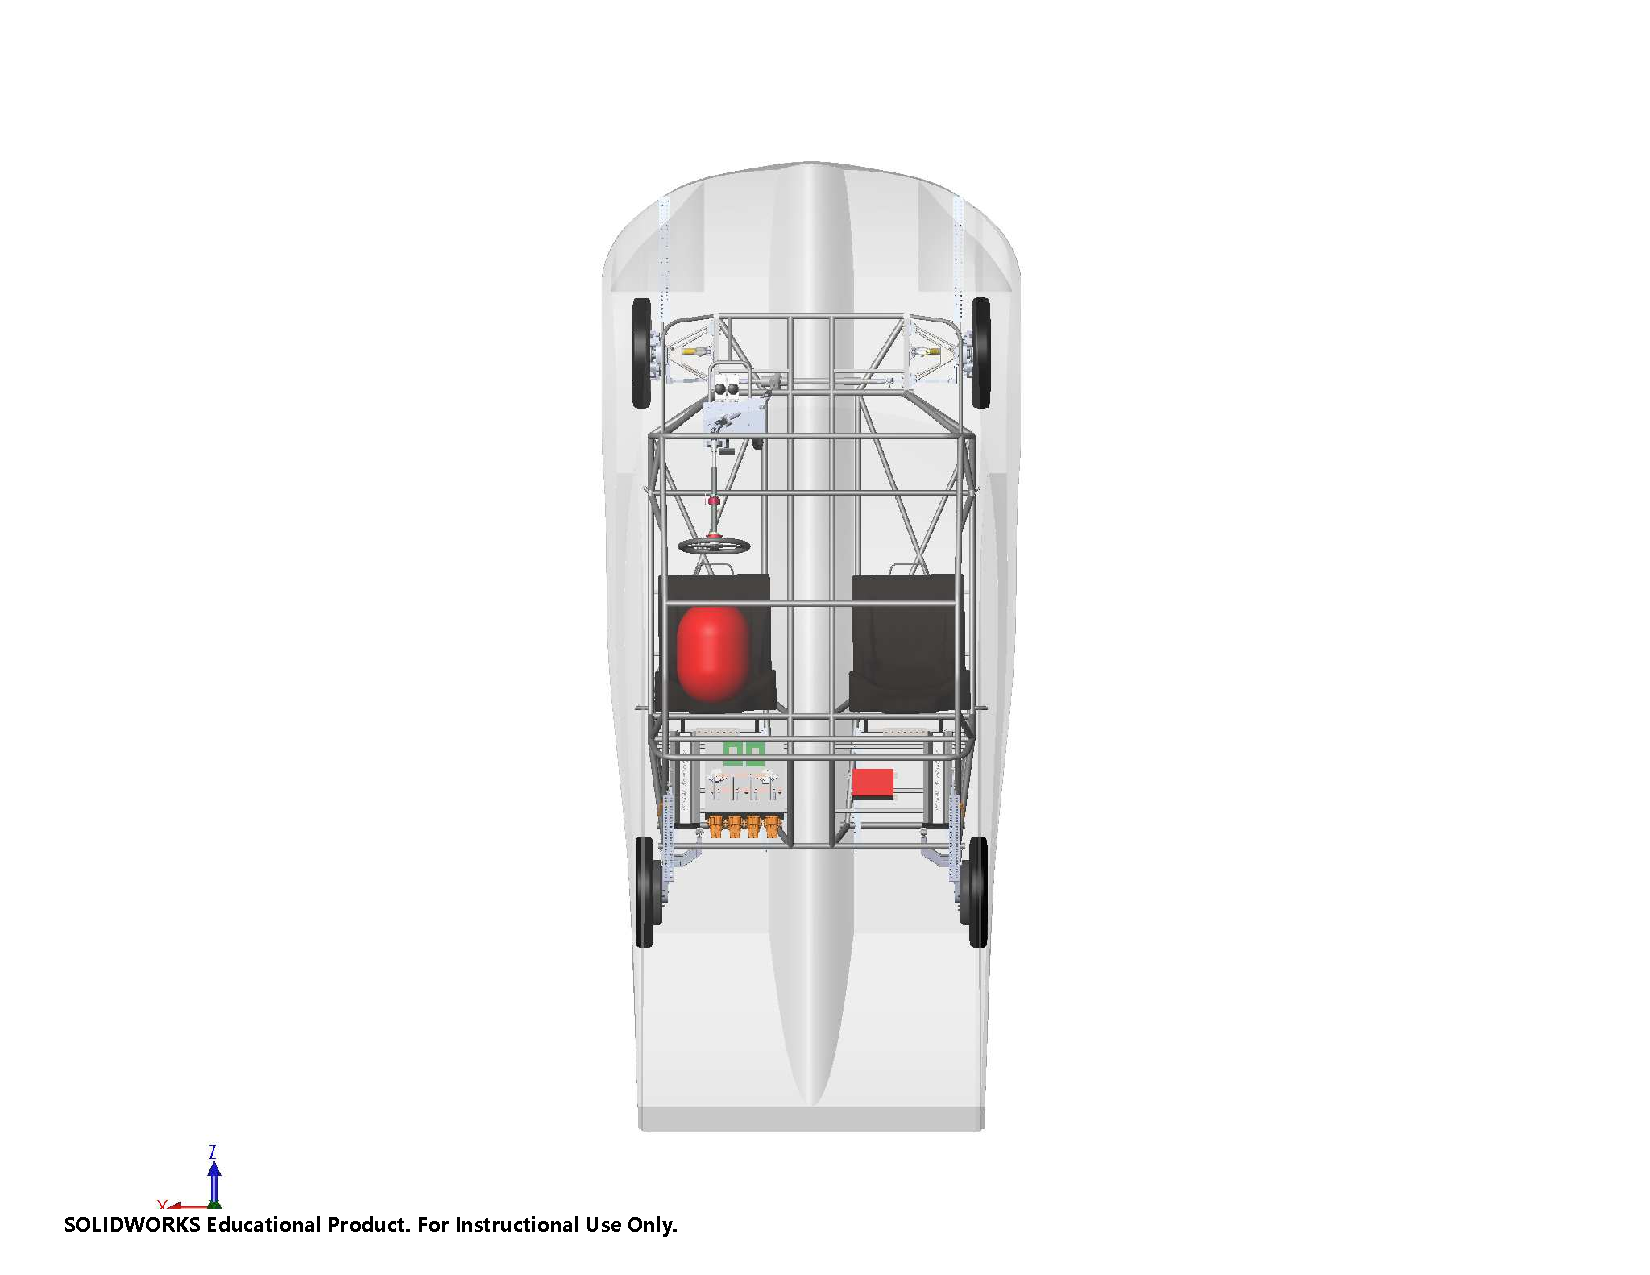
\includegraphics{figures/msxii-top-view}
\caption{Top view showing major dimensions and system positions}
\label{fig:msxii-top-view}
\end{figure}

\begin{figure}
\centering
%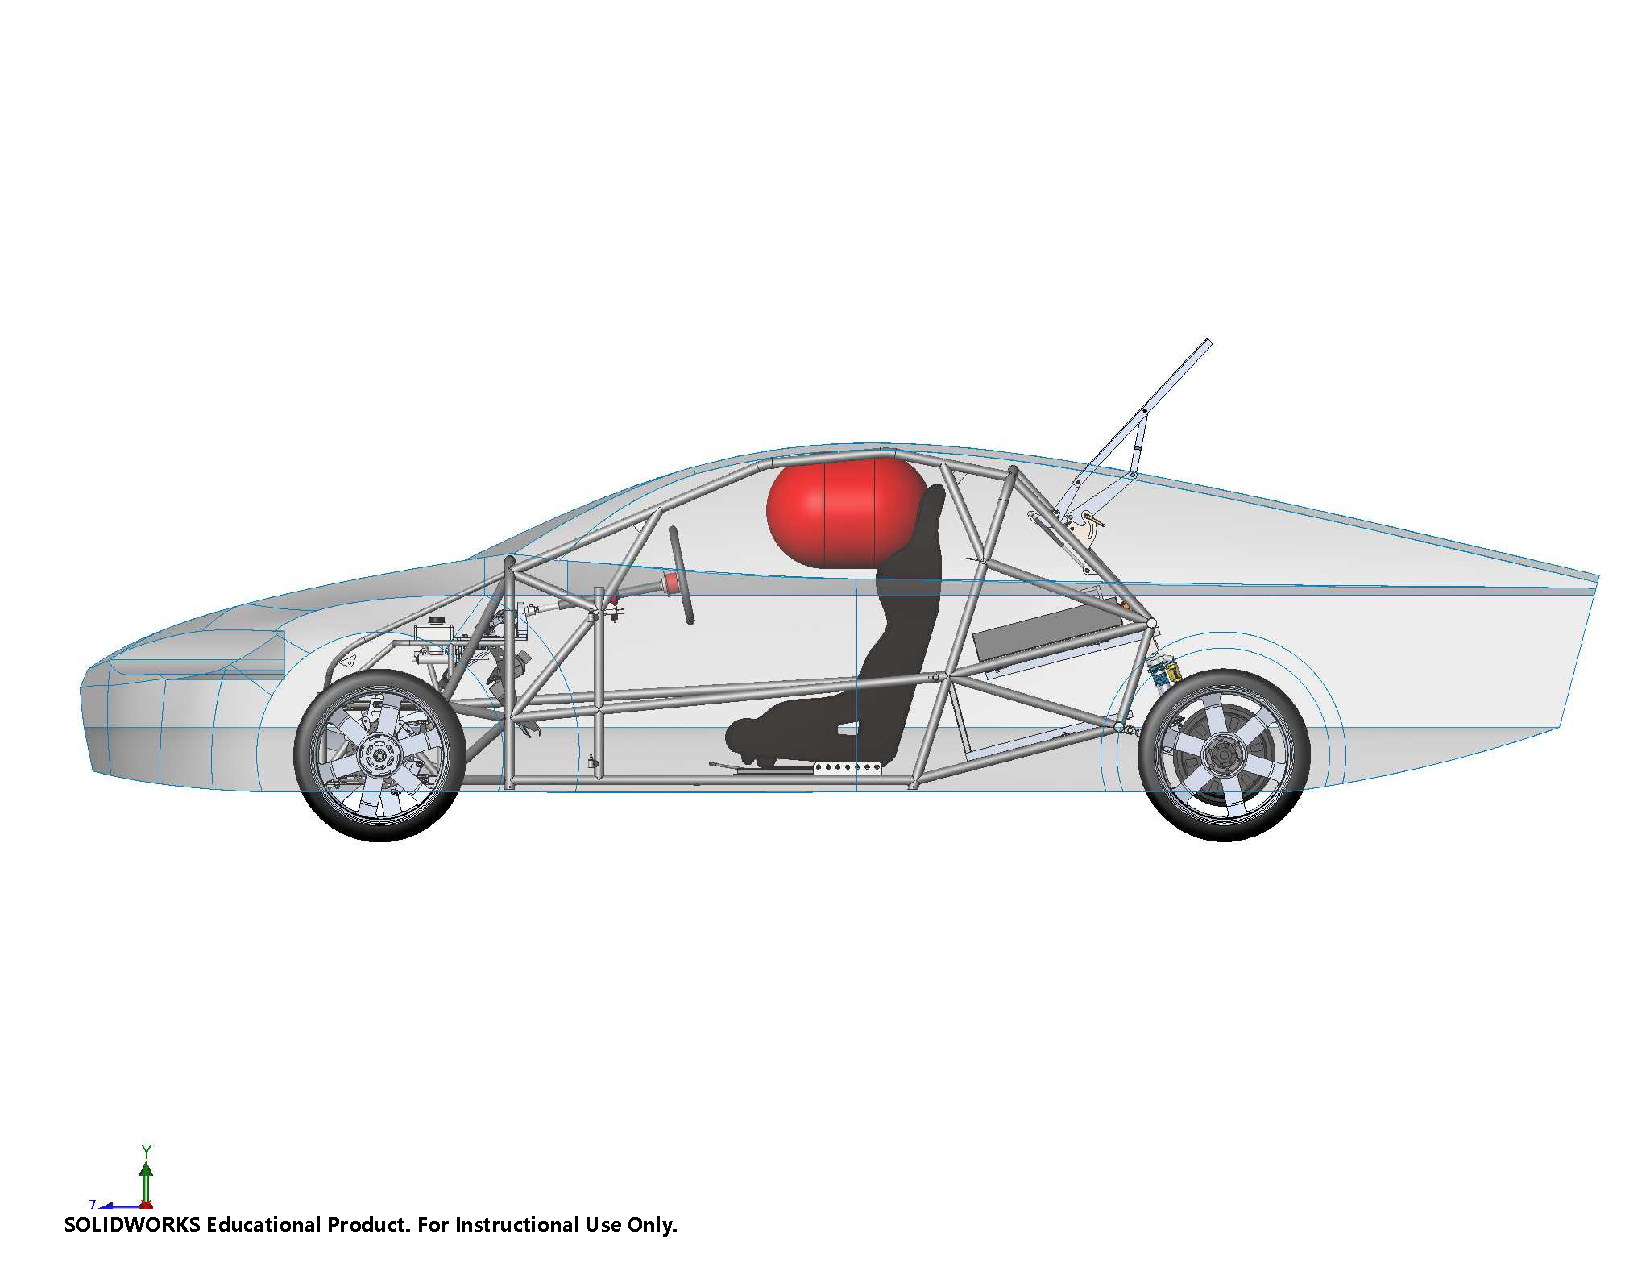
\includegraphics{figures/msxii-side-view}
\caption{Side view showing major dimensions and system positions}
\label{fig:msxii-side-view}
\end{figure}

\begin{table}
\centering
\begin{tabular}{cc}
\toprule
Parameter & Value \\
\midrule
Wheelbase & \SI{2.60}{\metre} \\
Track     & \SI{1.60}{\metre} \\
\bottomrule
\end{tabular}
\caption{Table of major vehicle dimensions}
\label{tab:msxii-dimensions}
\end{table}

\subsection{Chassis}
\subsubsection{Design}
The chassis is a tube structure enclosing the occupant cell with small front and rear subframes to support suspension hardpoints. Smaller non-structural tube members will extend from the main frame to provide support to body panels as necessary. The majority of tubes are round, with square tubes being used only for elements intended to mount suspension and powertrain components (battery pack, motor controllers). Chassis elements use SAE 4130N chromoly tubes with diameters or side lengths ranging from 0.750" to 1.250", and wall thicknesses ranging from 0.035" to 0.065". Isometric drawings of the chassis are shown in Figures \ref{fig:chassis-front}, \ref{fig:chassis-top}, and \ref{fig:chassis-side}.

\begin{figure}
\centering
%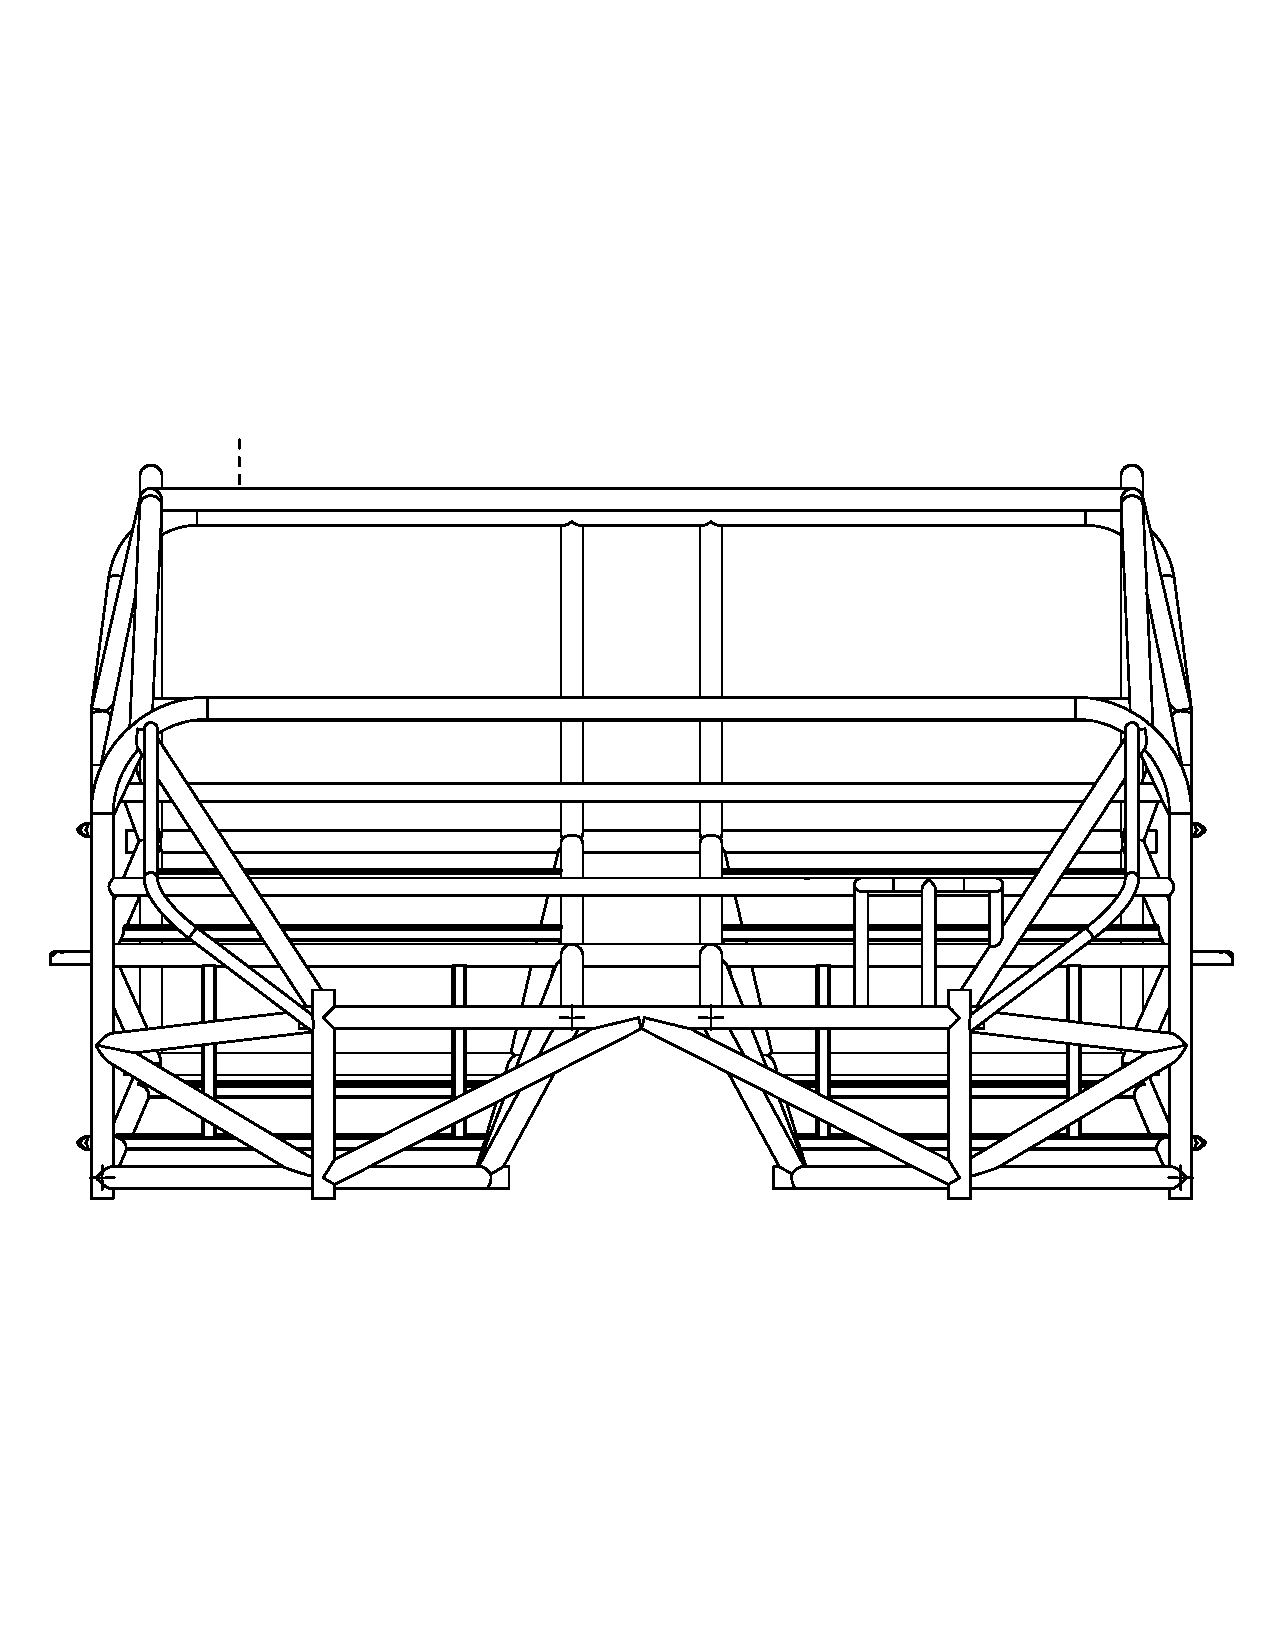
\includegraphics{figures/chassis-front}
\caption{Chassis, front view}
\label{fig:chassis-front}
\end{figure}
\begin{figure}
\centering
%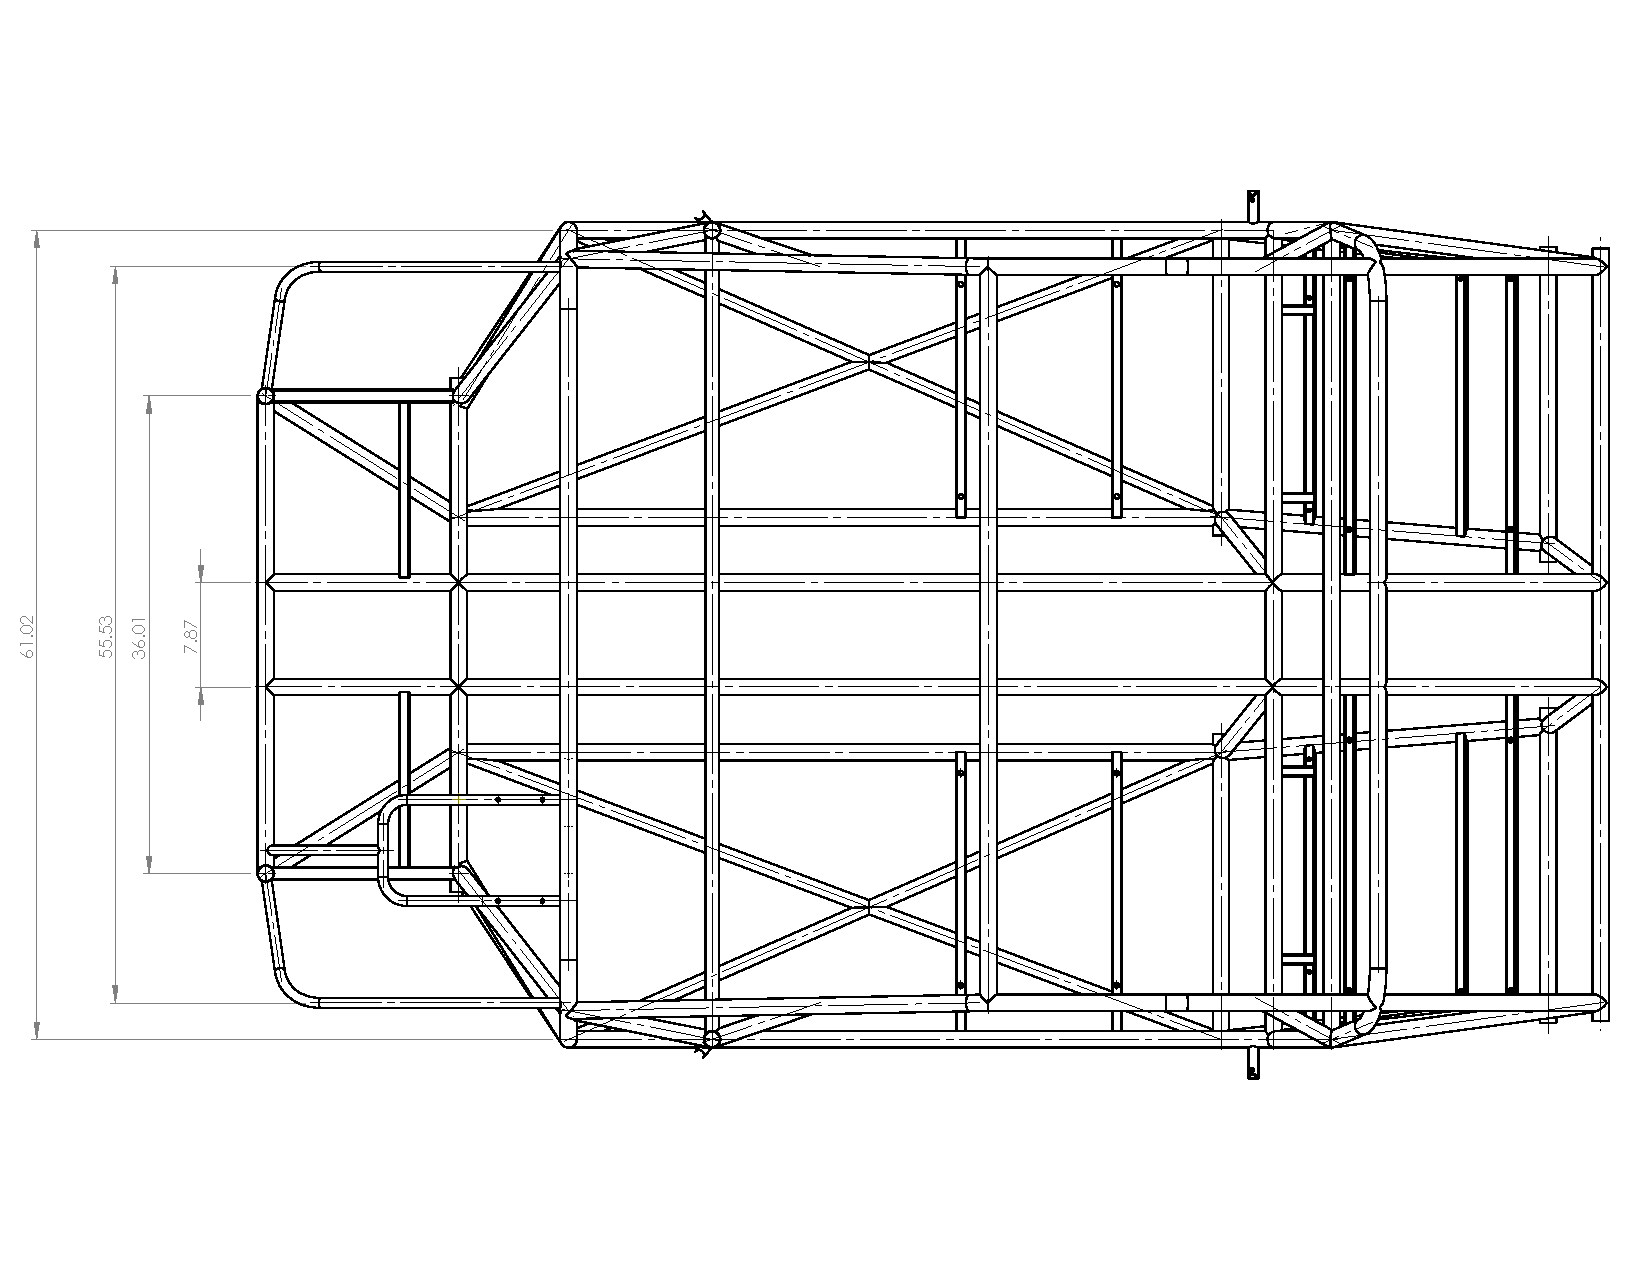
\includegraphics{figures/chassis-top}
\caption{Chassis, top view}
\label{fig:chassis-top}
\end{figure}
\begin{figure}
\centering
%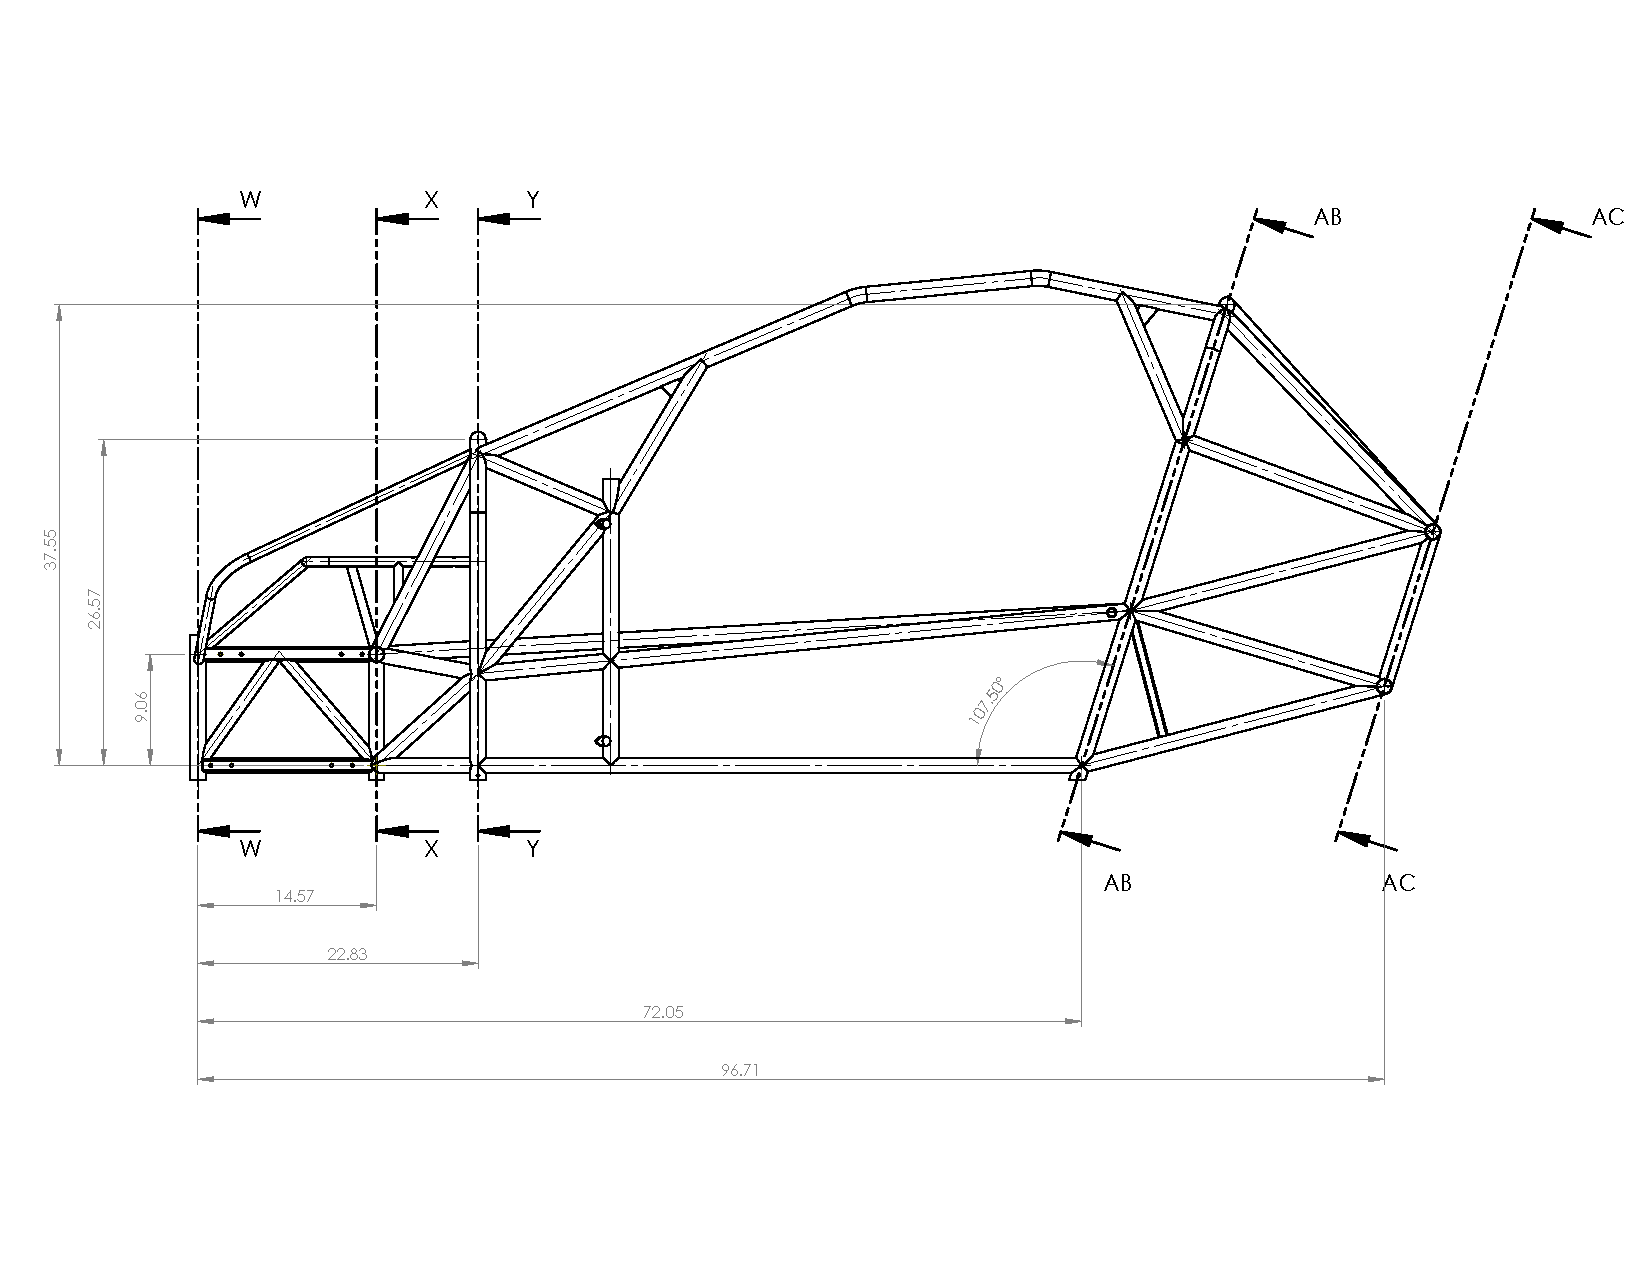
\includegraphics{figures/chassis-side}
\caption{Chassis, side view}
\label{fig:chassis-side}
\end{figure}

\subsubsection{Manufacturing}
Bending, cutting, and profiling of tubes was done by an external supplier. Welding of the chassis was done by a professional welder using GTAW, with support from team members for jigging and assembly. A complete welding jig was designed in CAD and manufactured using 80/20 aluminum extrusion tubing, shown in Figure \ref{fig:welding-jig}. Custom tube clamps were machined by the team to slot into jig members and fully support all chassis elements through multiple stages of assembly and welding.

\begin{figure}
\centering
%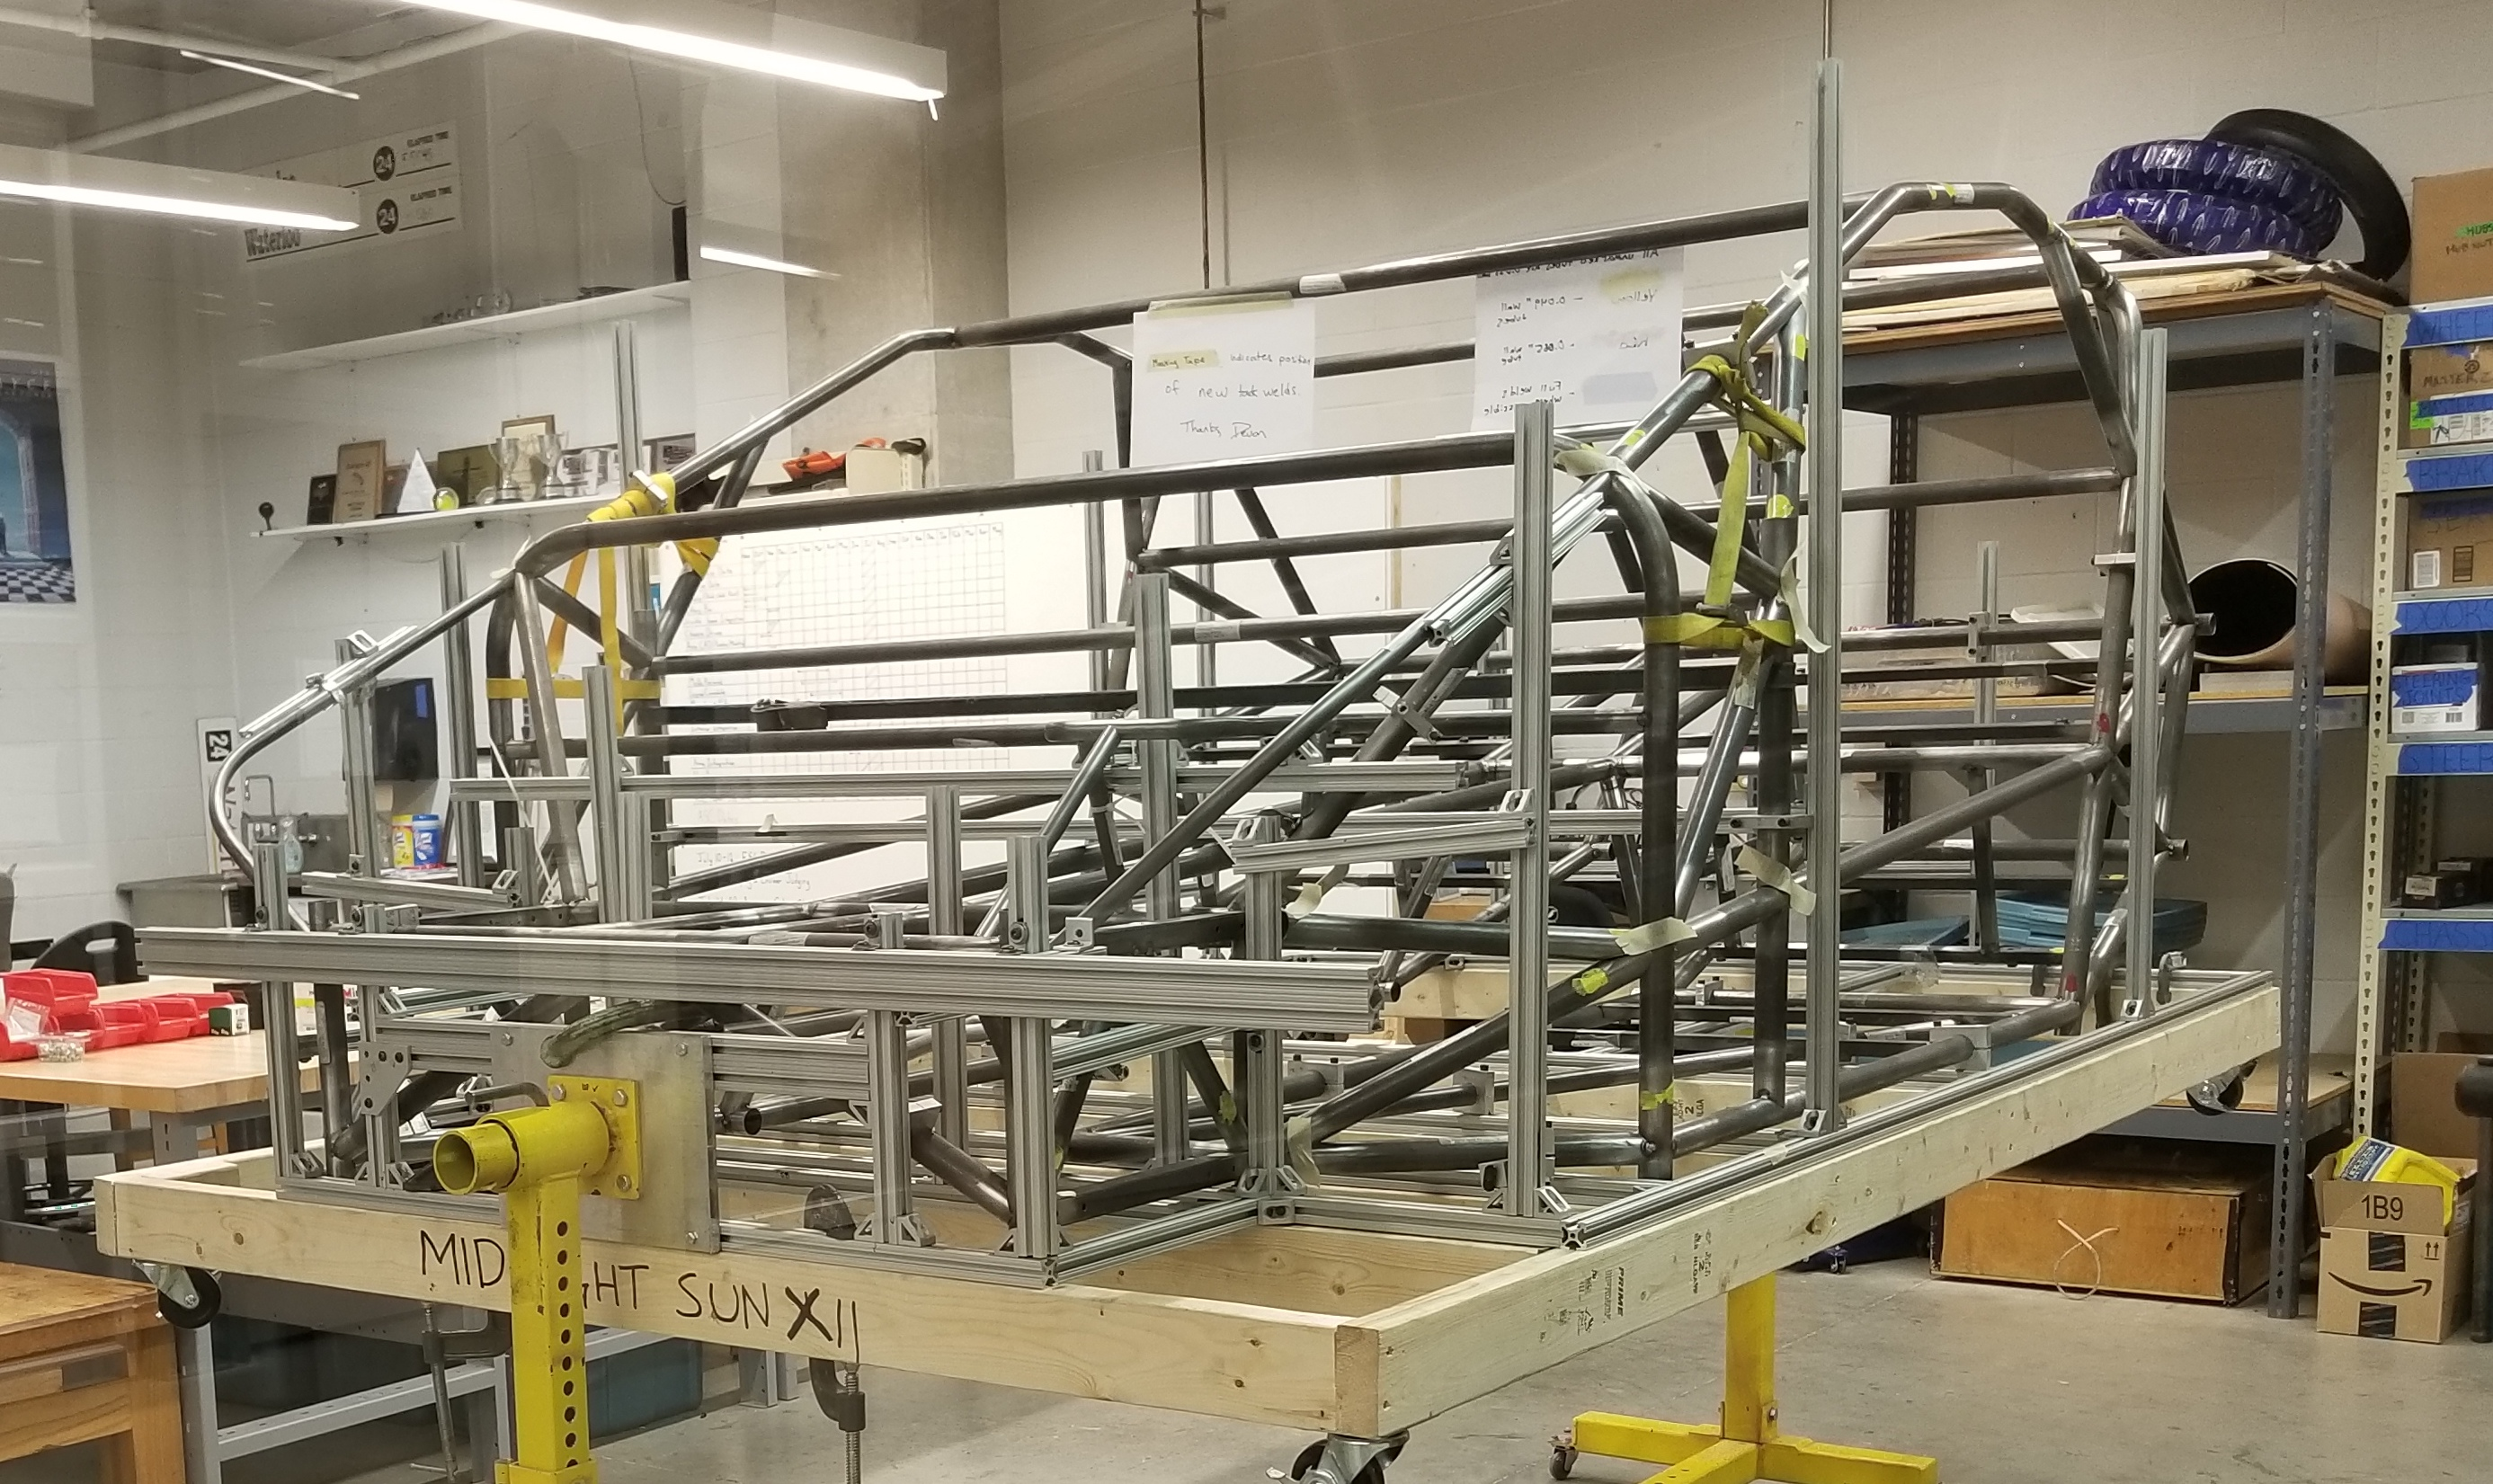
\includegraphics{figures/welding-jig}
\caption{Welding jig under construction}
\label{fig:welding-jig}
\end{figure}

\subsubsection{Roll cage}
The roll cage is integrated into the design of the chassis members enclosing the occupant cell. For the purposes of ASC regulations, the roll cage can be considered to include the A and B pillar hoops and elements connecting these two hoops lengthwise through the car. For clarity, these elements have been highlighted in Figure \ref{fig:roll-cage}.

\begin{figure}
\centering
%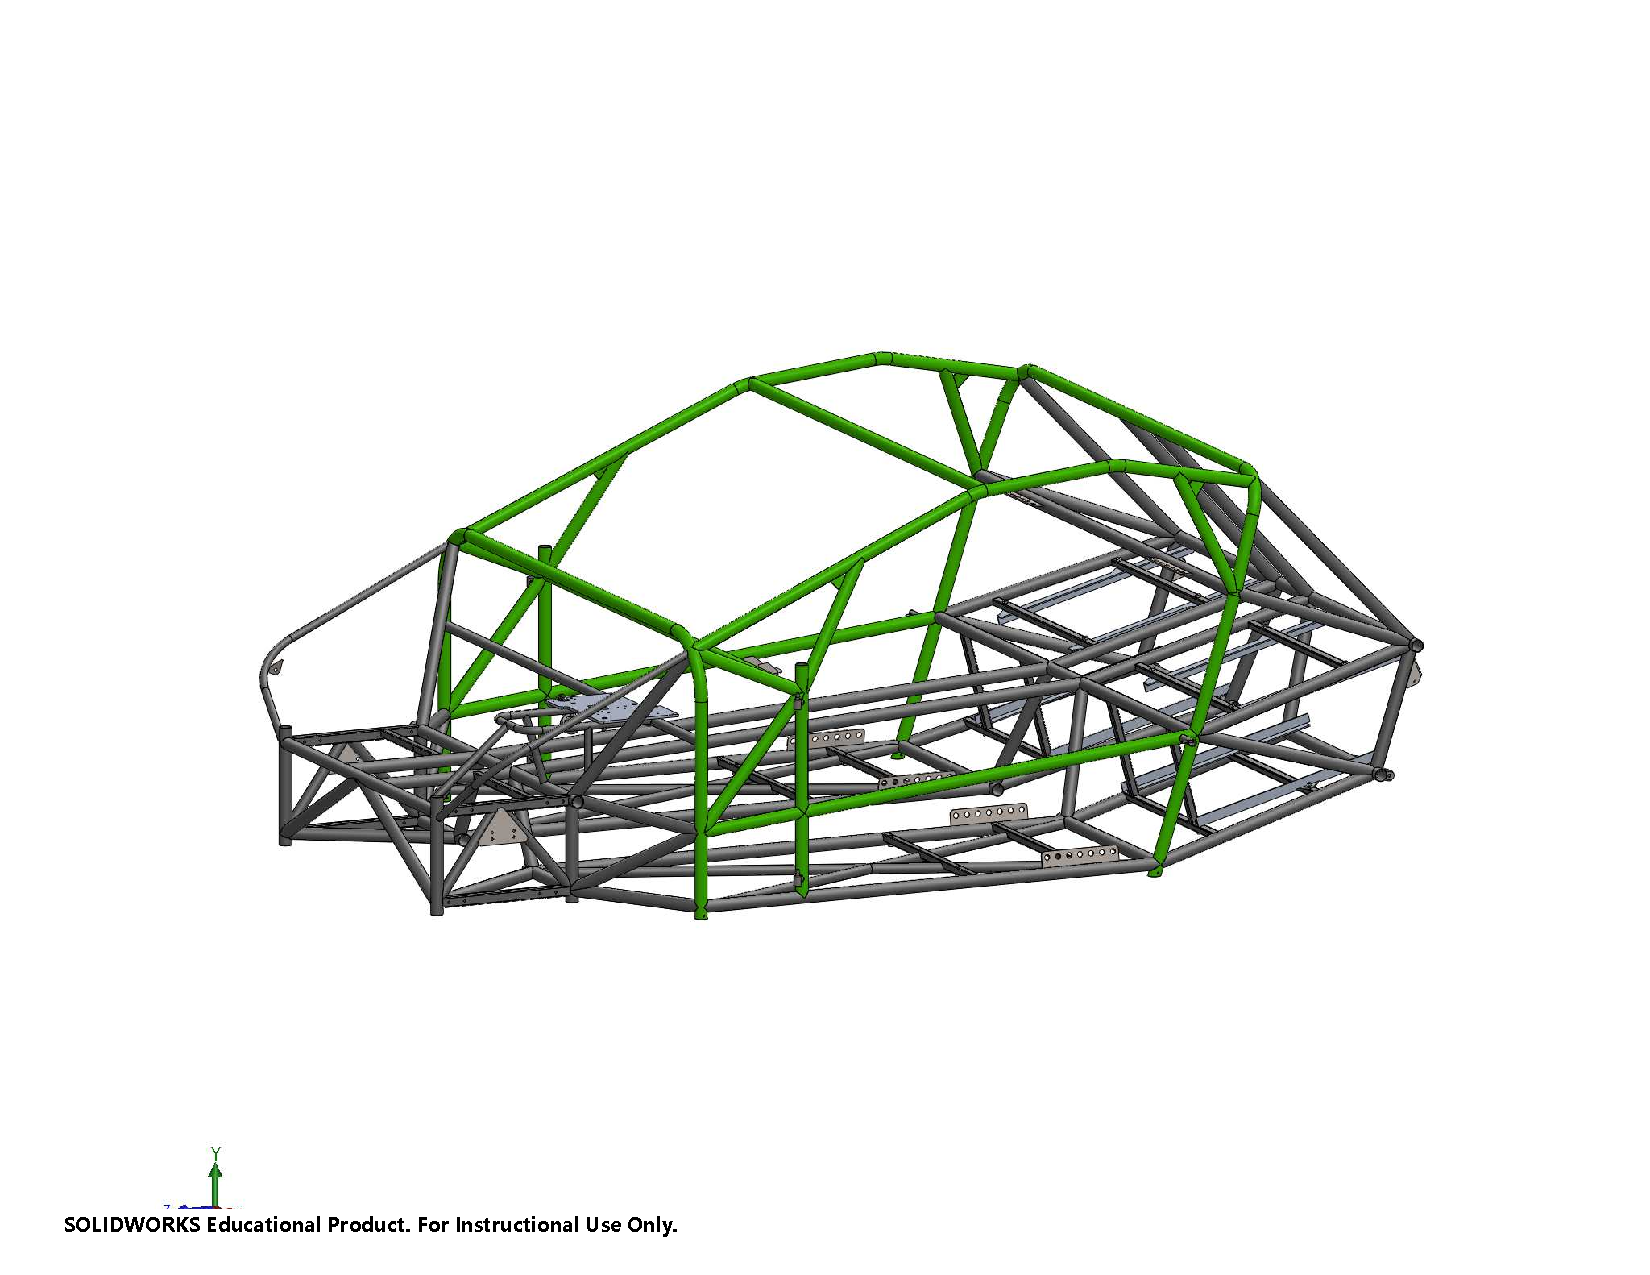
\includegraphics{figures/roll-cage}
\caption{Chassis with roll cage elements highlighted}
\label{fig:roll-cage}
\end{figure}


\subsection{Seat Belts}
MSXII is equipped with 5-point seat belts for both occupants. Seat belt hardpoints are mounted to metal tabs welded to chassis members, shown in Figure \ref{fig:seat-belt-tab-positions}. Figure \ref{fig:seat-belt-tab} shows one of these tabs. Figures \ref{fig:seat-belt-side-view} and \ref{fig:seat-belt-top-view} demonstrate compliance with ASC regulations 10.3.E.

\begin{figure}
\centering
%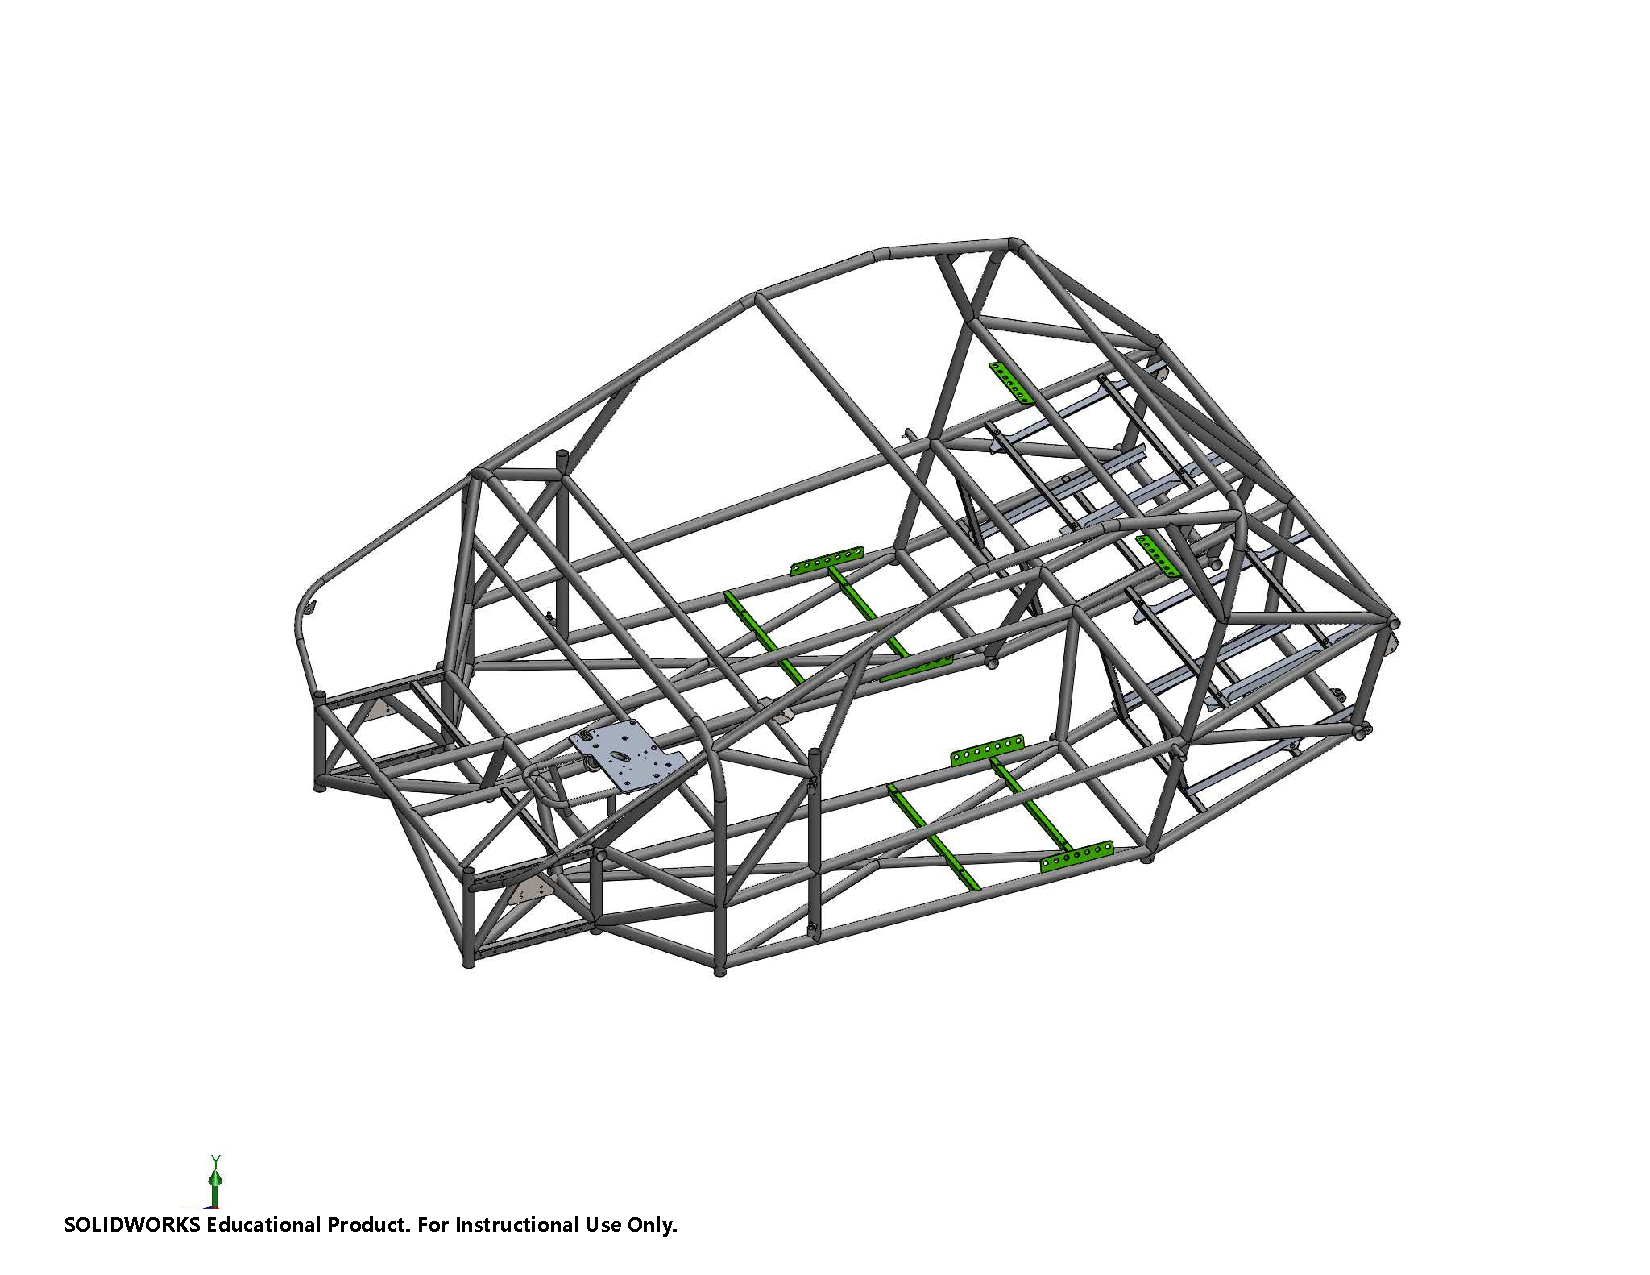
\includegraphics{figures/seat-belt-tab-positions}
\caption{Chassis mounting points for seat belts}
\label{fig:seat-belt-tab-positions}
\end{figure}

\begin{figure}
\centering
%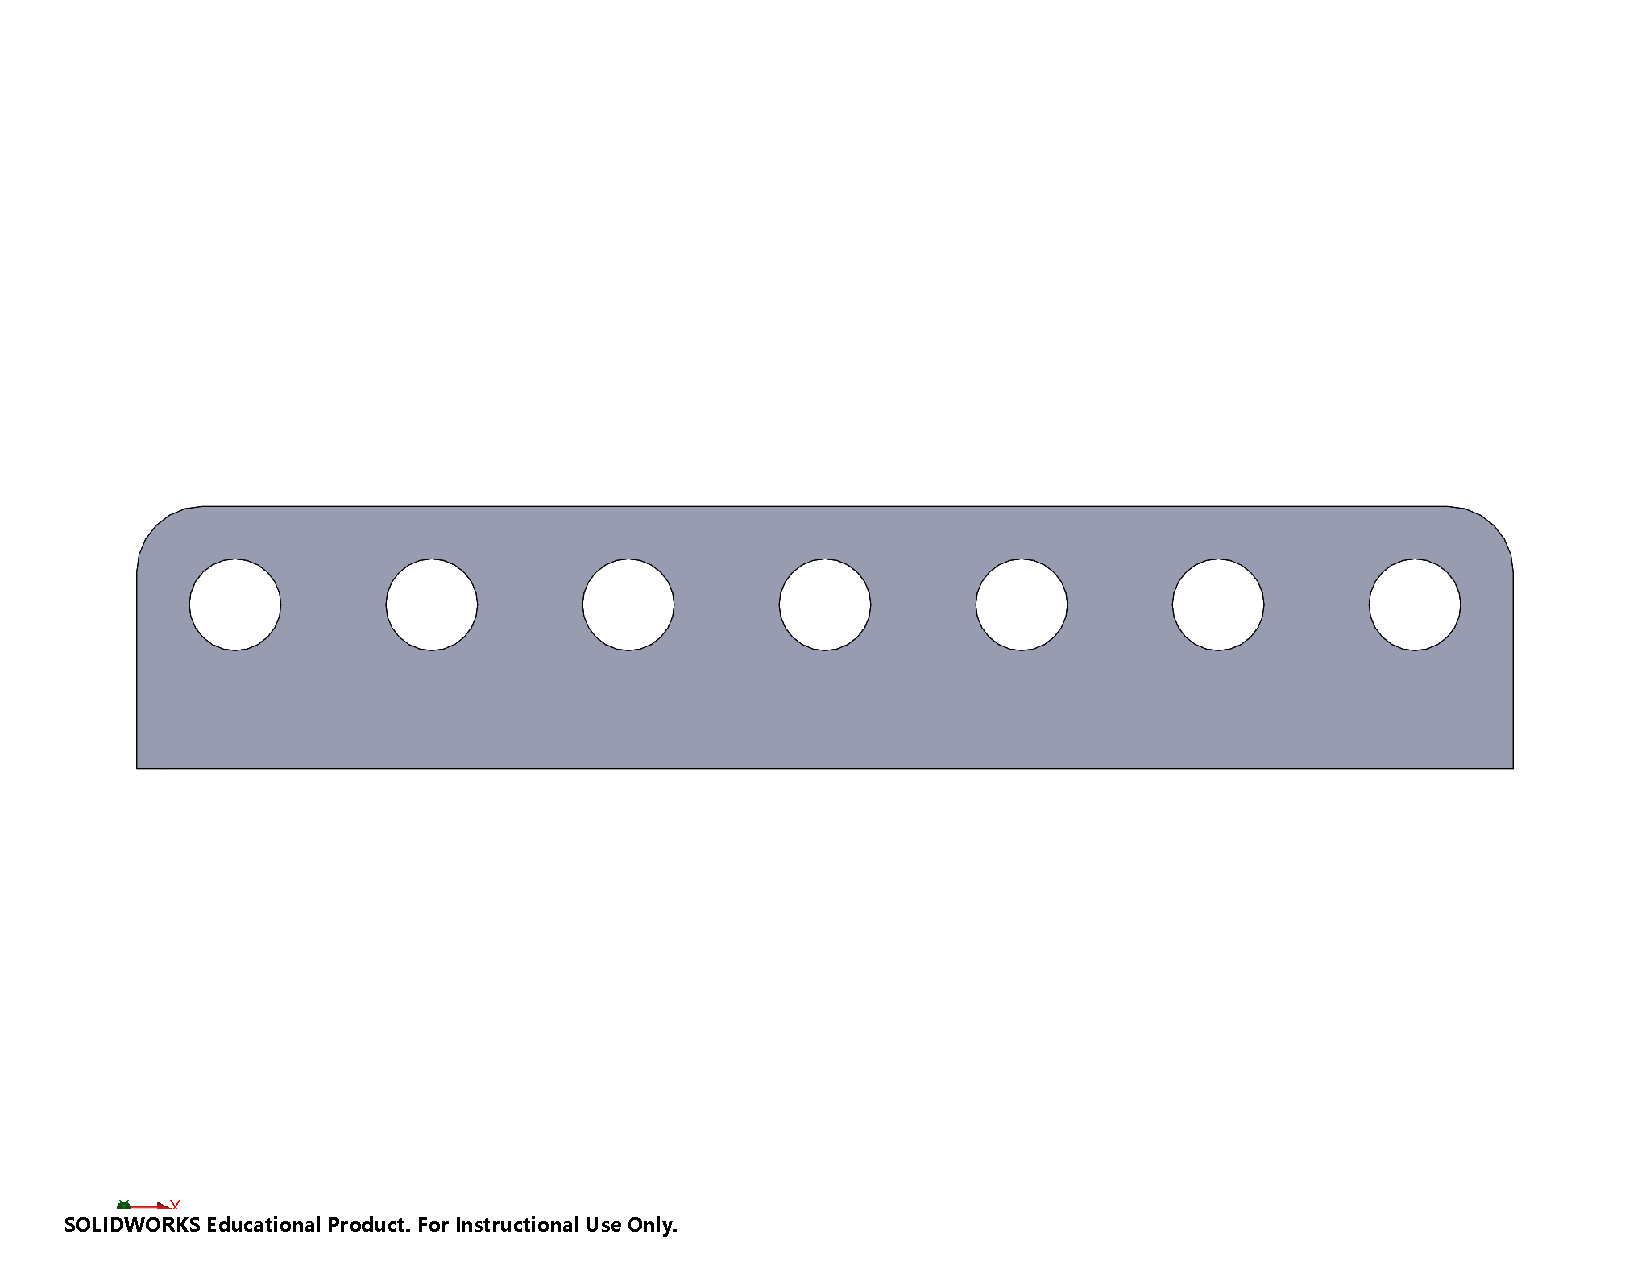
\includegraphics{figures/seat-belt-tab}
\caption{Single seat belt tab}
\label{fig:seat-belt-tab}
\end{figure}

\begin{figure}
\centering
%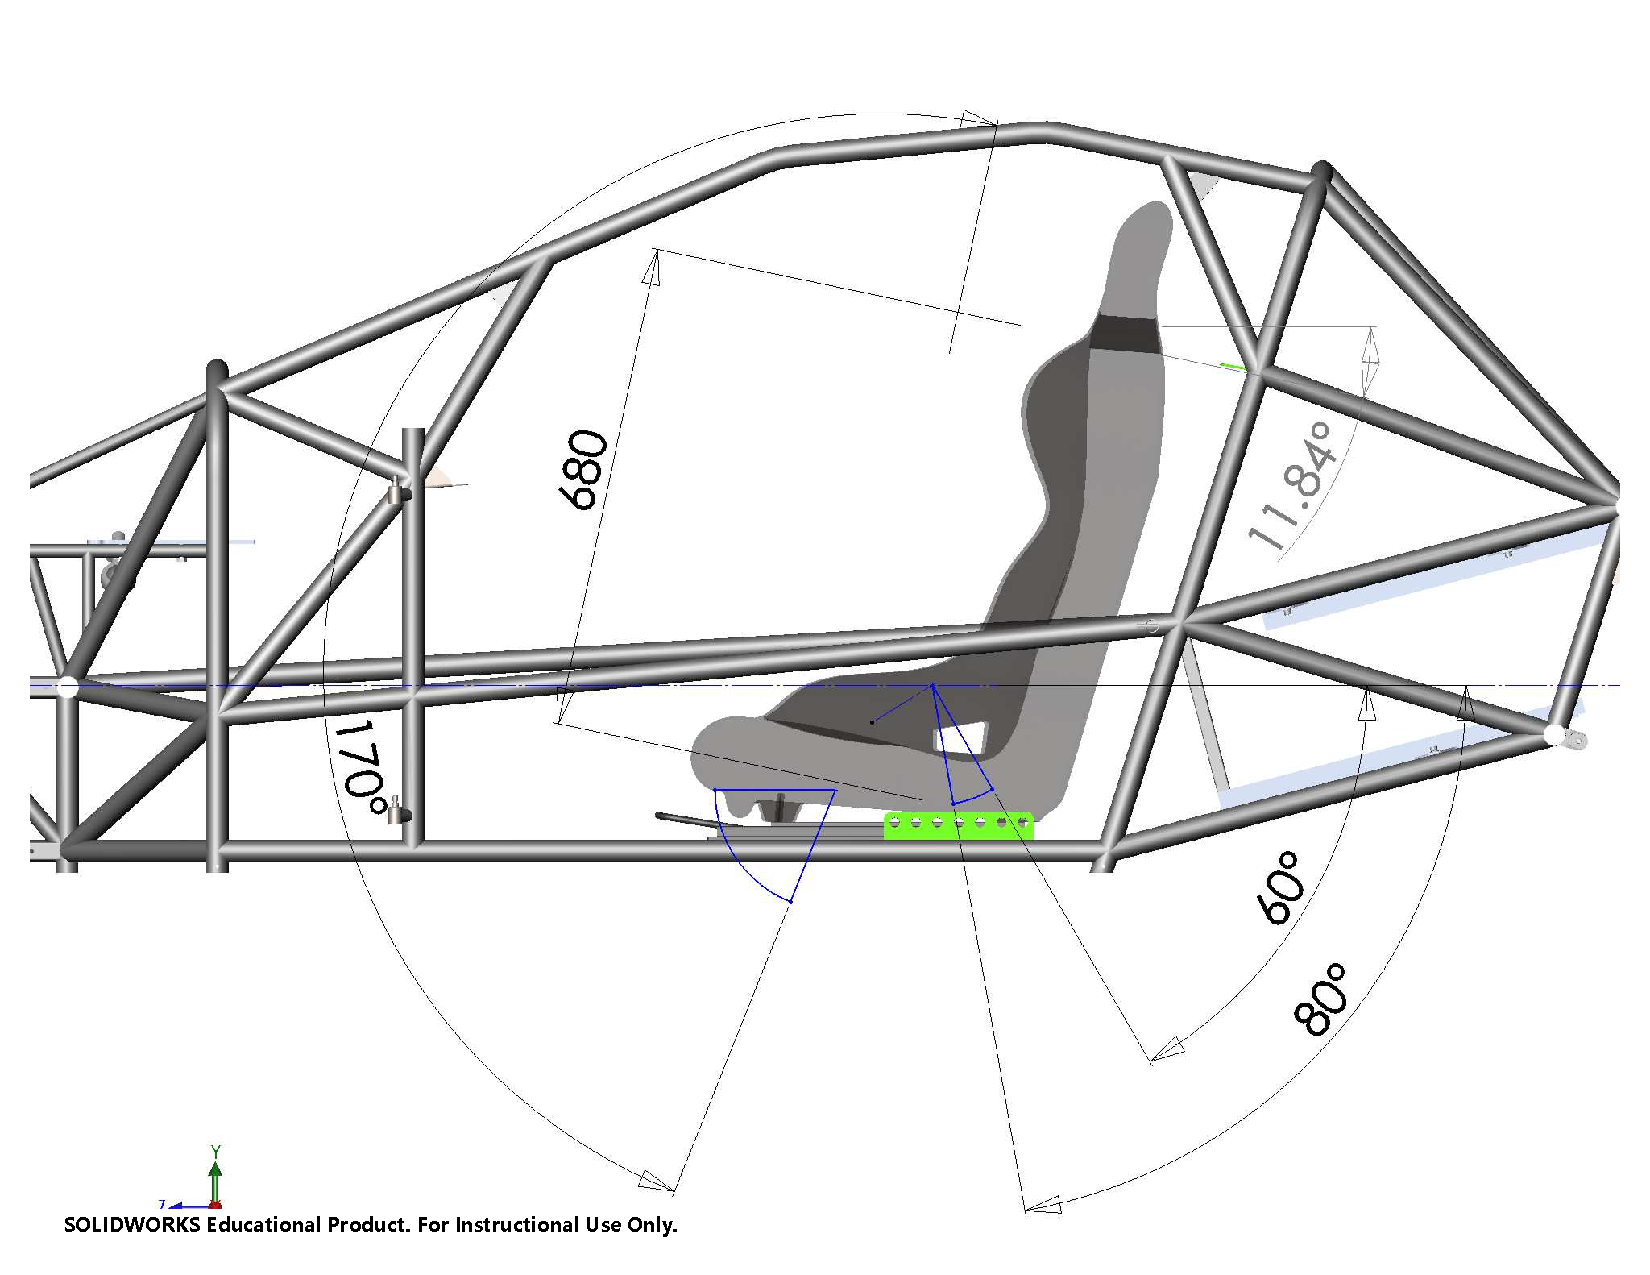
\includegraphics{figures/seat-belt-side-view}
\caption{Side view of seat belt geometry}
\label{fig:seat-belt-side-view}
\end{figure}

\begin{figure}
\centering
%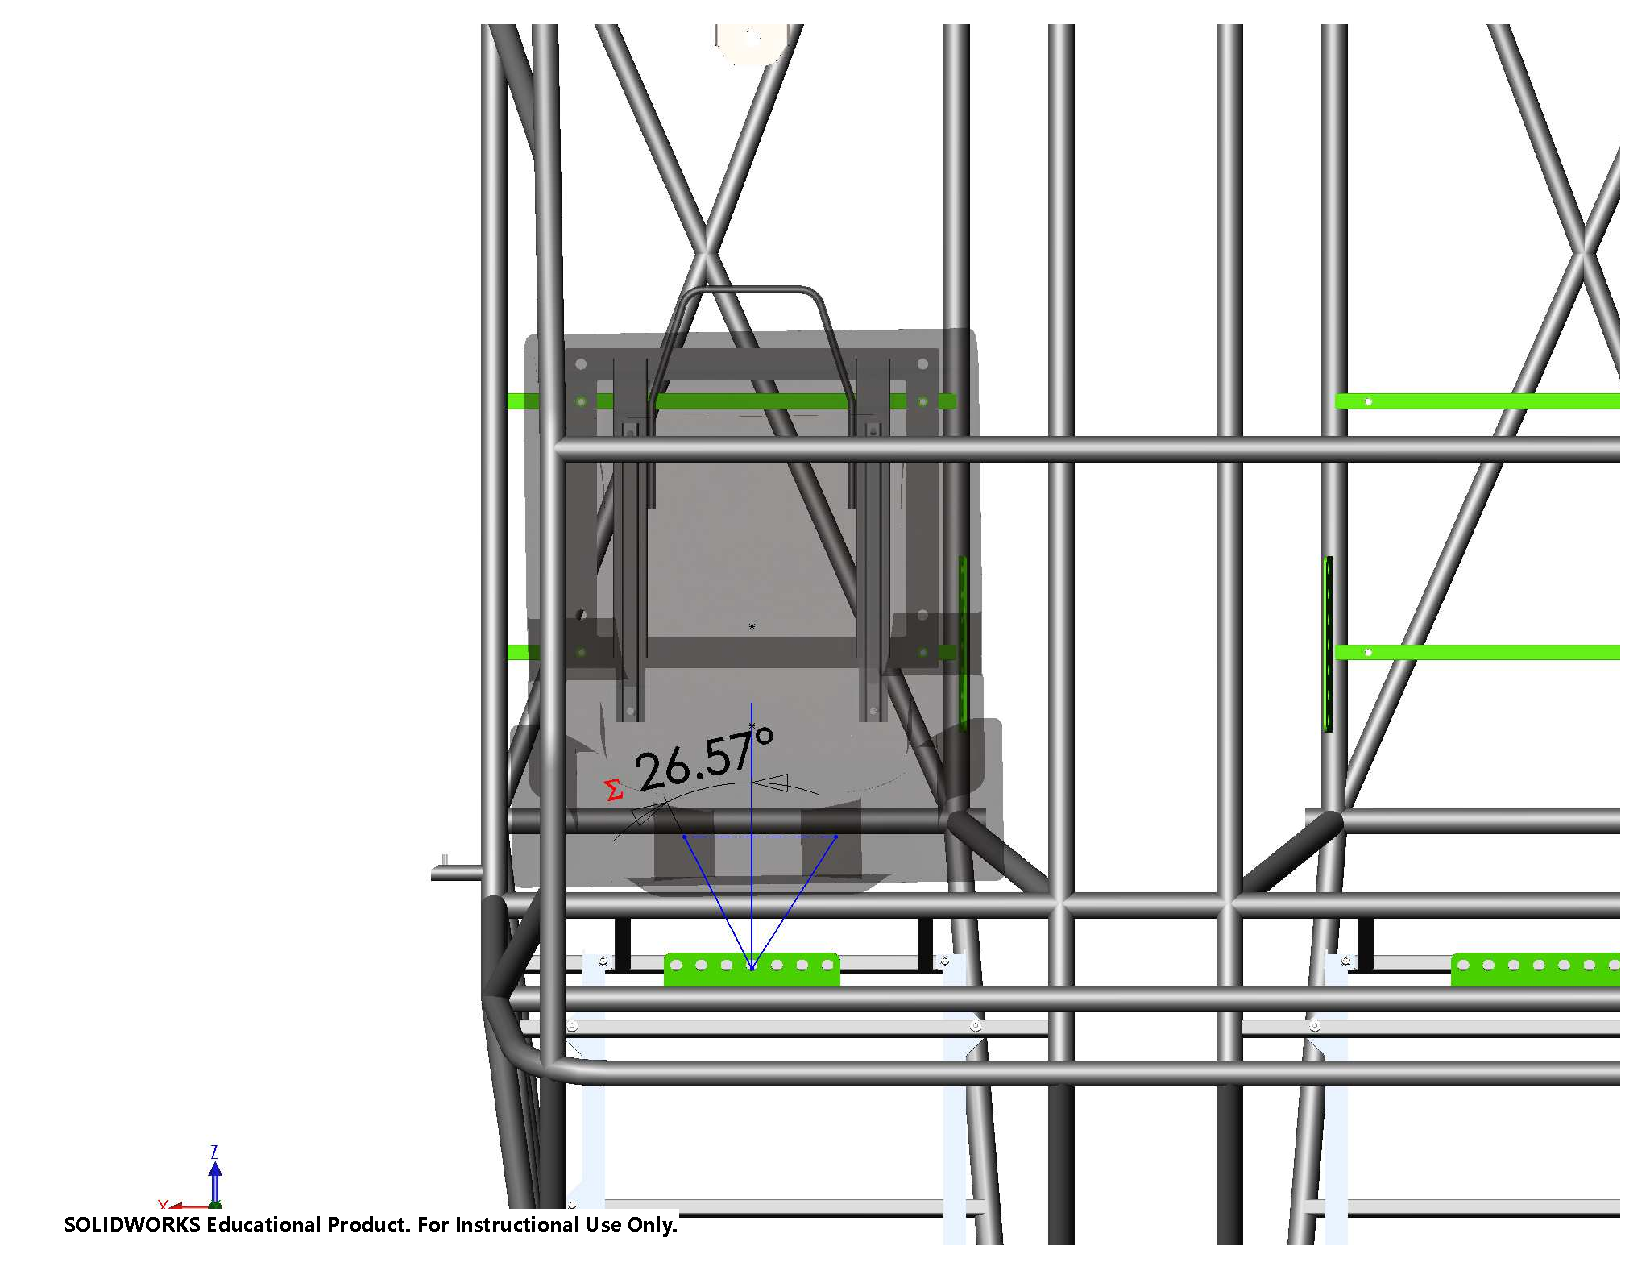
\includegraphics{figures/seat-belt-top-view}
\caption{Top view of seat belt geometry}
\label{fig:seat-belt-top-view}
\end{figure}

\subsection{Braking System}
\subsubsection{Primary Brakes}
The primary braking system is designed with dual redundant front braking, consisting of two identical systems with separate master cylinders, hydraulic lines, and calipers to each of the left and right wheels. The master cylinders are operated in unision via a single mechanical brake pedal. A schematic of the primary system is shown in Figure \ref{fig:primary-brakes-schematic}.

\begin{figure}
\centering
%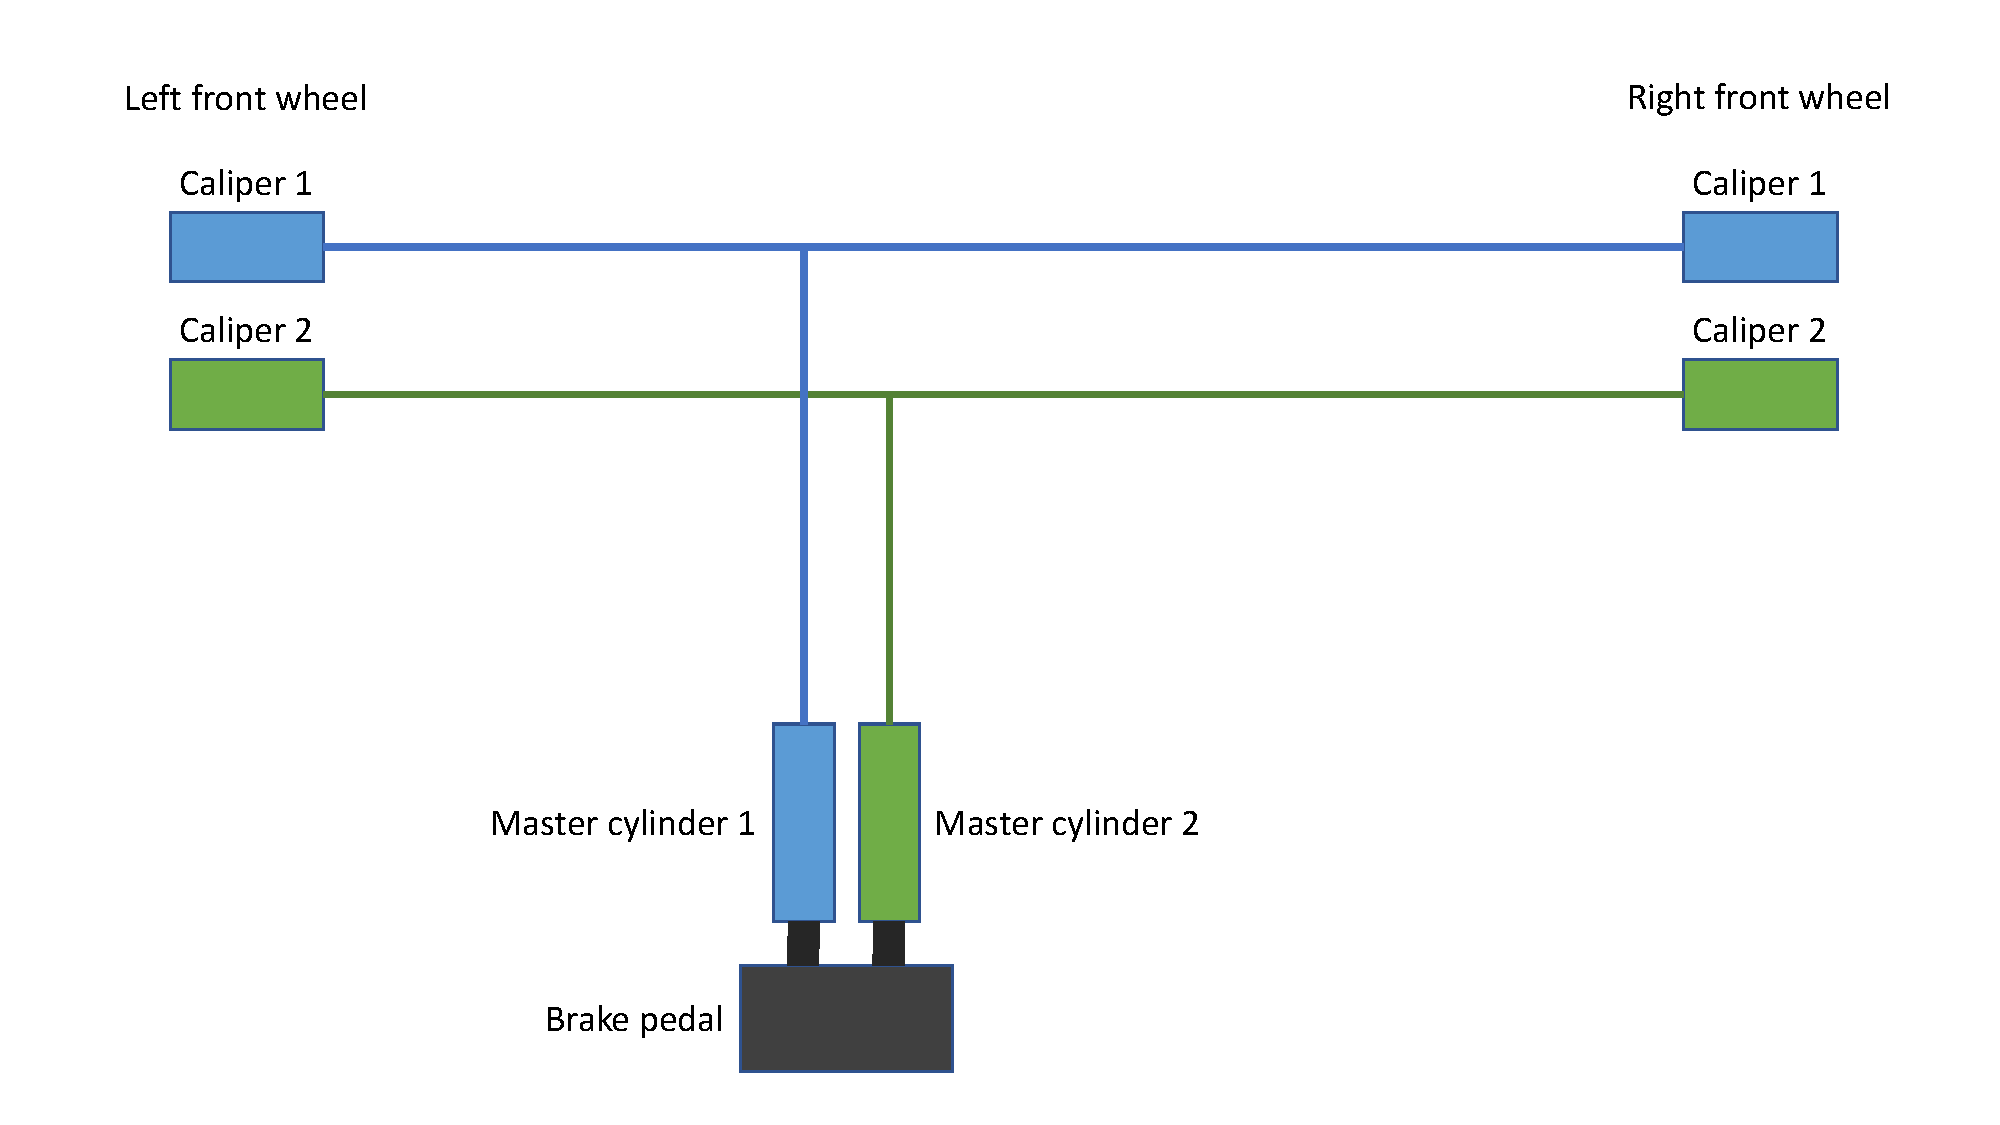
\includegraphics{figures/primary-brakes-schematic}
\caption{Schematic of primary braking system}
\label{fig:primary-brakes-schematic}
\end{figure}

Front brake calipers are Willwood parts \href{http://www.wilwood.com/Calipers/CaliperProd.aspx?itemno=120-8374}{120-8374} (left) and \href{http://www.wilwood.com/Calipers/CaliperProd.aspx?itemno=120-8373}{120-8373} (right). Willwood's website indicates the caliper pads have \SI{2}{in\squared} (\SI{12.9}{\centi\metre\squared}) contact area and 0.30" (\SI{7.6}{\milli\metre}) depth including the backing plate.

The master cylinders are Willwood part \href{http://www.wilwood.com/MasterCylinders/MasterCylinderProd.aspx?itemno=260-3374}{206-3374}. They have a 3/8"-24 outlet size which will need to be connected via an adapter to the M10 x 1.25 inlets of the calipers. Brake lines will be DOT-approved hose assemblies sized for 3/8"-24. The brake pedal is Willwood part \href{http://www.wilwood.com/Pedals/PedalProd.aspx?itemno=340-15079}{340-15079} and is mounted in the standard configuration to the left of the accelerator pedal.

Brake rotors will be custom-machined within the supported disk thickness and diameter supported by the Willwood calipers. All mounting geometry on the suspension upright for primary calipers are designed to position the primary calipers in the optimal positions to meet braking specifications.

\subsubsection{Parking Brake}
The parking brake will be implemented by a cable-actuated caliper mounted at one of the front wheels. The caliper is the Tolomatic ME10LA, part number \href{https://www.tolomatic.com/products/product-details/me10-mechanical-disc-brake#/specs-order}{0732-0003}. It will share the same brake disk as the primary braking system but is otherwise mechanically independent. Due to unresolvable dimensioning differences between the Tolomatic and Willwood calipers, the parking brake caliper cannot be mounted perfectly as per the manufacturer's recommendations and will have only 80\% overlap with the brake disk. However, this is expected to provide more than sufficient countertorque to keep the vehicle stationary as per ASC regulations 10.6.

Figure \ref{fig:calipers-mounting-geometry} shows a front suspension upright with all three calipers mounted (two primary and one parking).

\begin{figure}
\centering
%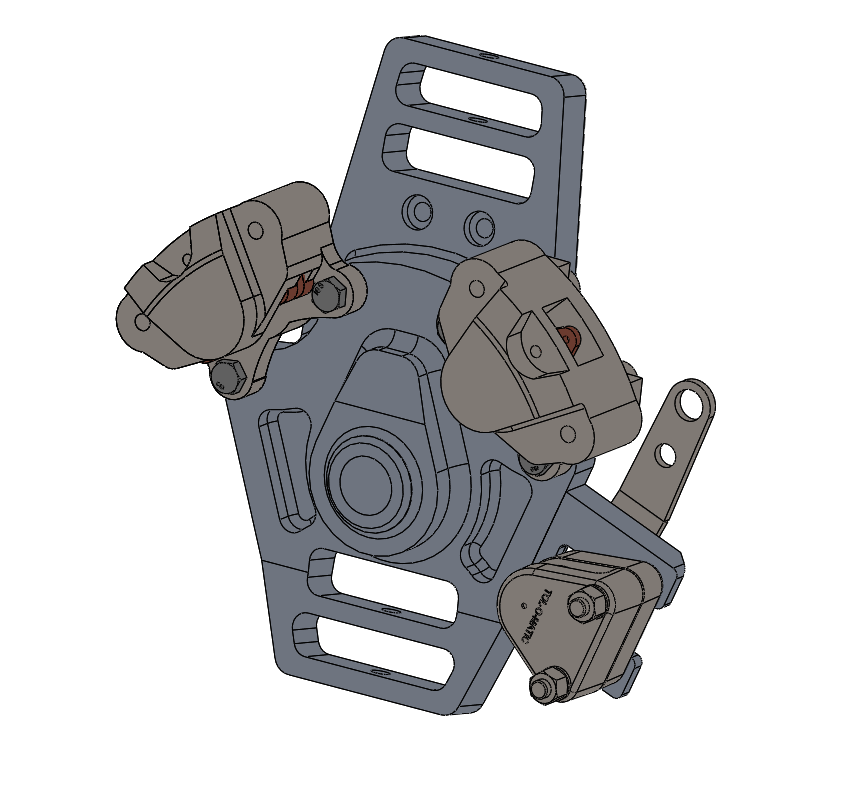
\includegraphics{figures/caliper-mounting-geometry}
\caption{View of dual-primary and parking calipers on front suspension upright }
\label{fig:calipers-mounting-geometry}
\end{figure}

\subsection{Steering System}
The steering system uses a rear-steering, left-hand-drive rack and pinion from Helix (part number \href{http://www.helixsuspension.com/catalog/Steering/Manual-Steering-Racks/HEXSR5/Omni-Manual-Steering-Rack---Rear-Steering}{188754}). 

The system uses a collapsible steering column from Sweet Mfg.\@, part number \href{https://sweetmfg.biz/product.php?productid=2836}{405-10310}. The steering system linkage uses multiple U-joints and is shown in Figure \ref{fig:steering-system}.

\begin{figure}
\centering
%\includegraphics{figures/steering-system}
\caption{View of linkage from steering column to rack and pinion}
\label{fig:steering-system}
\end{figure}

\subsection{Suspension}
\subsubsection{Front Suspension}
The front suspension uses dual A-arms with an outboard dampener and coilover spring. The upper and lower control arms are custom-built from 4130 chromoly tubes. The dampener and coilover are a single integrated assembly supplied by \"Ohlins, sold as the TTX25, which is marketed for Formula SAE vehicles. Figure \ref{fig:front-suspension} shows the front suspension assembly.

\begin{figure}
\centering
%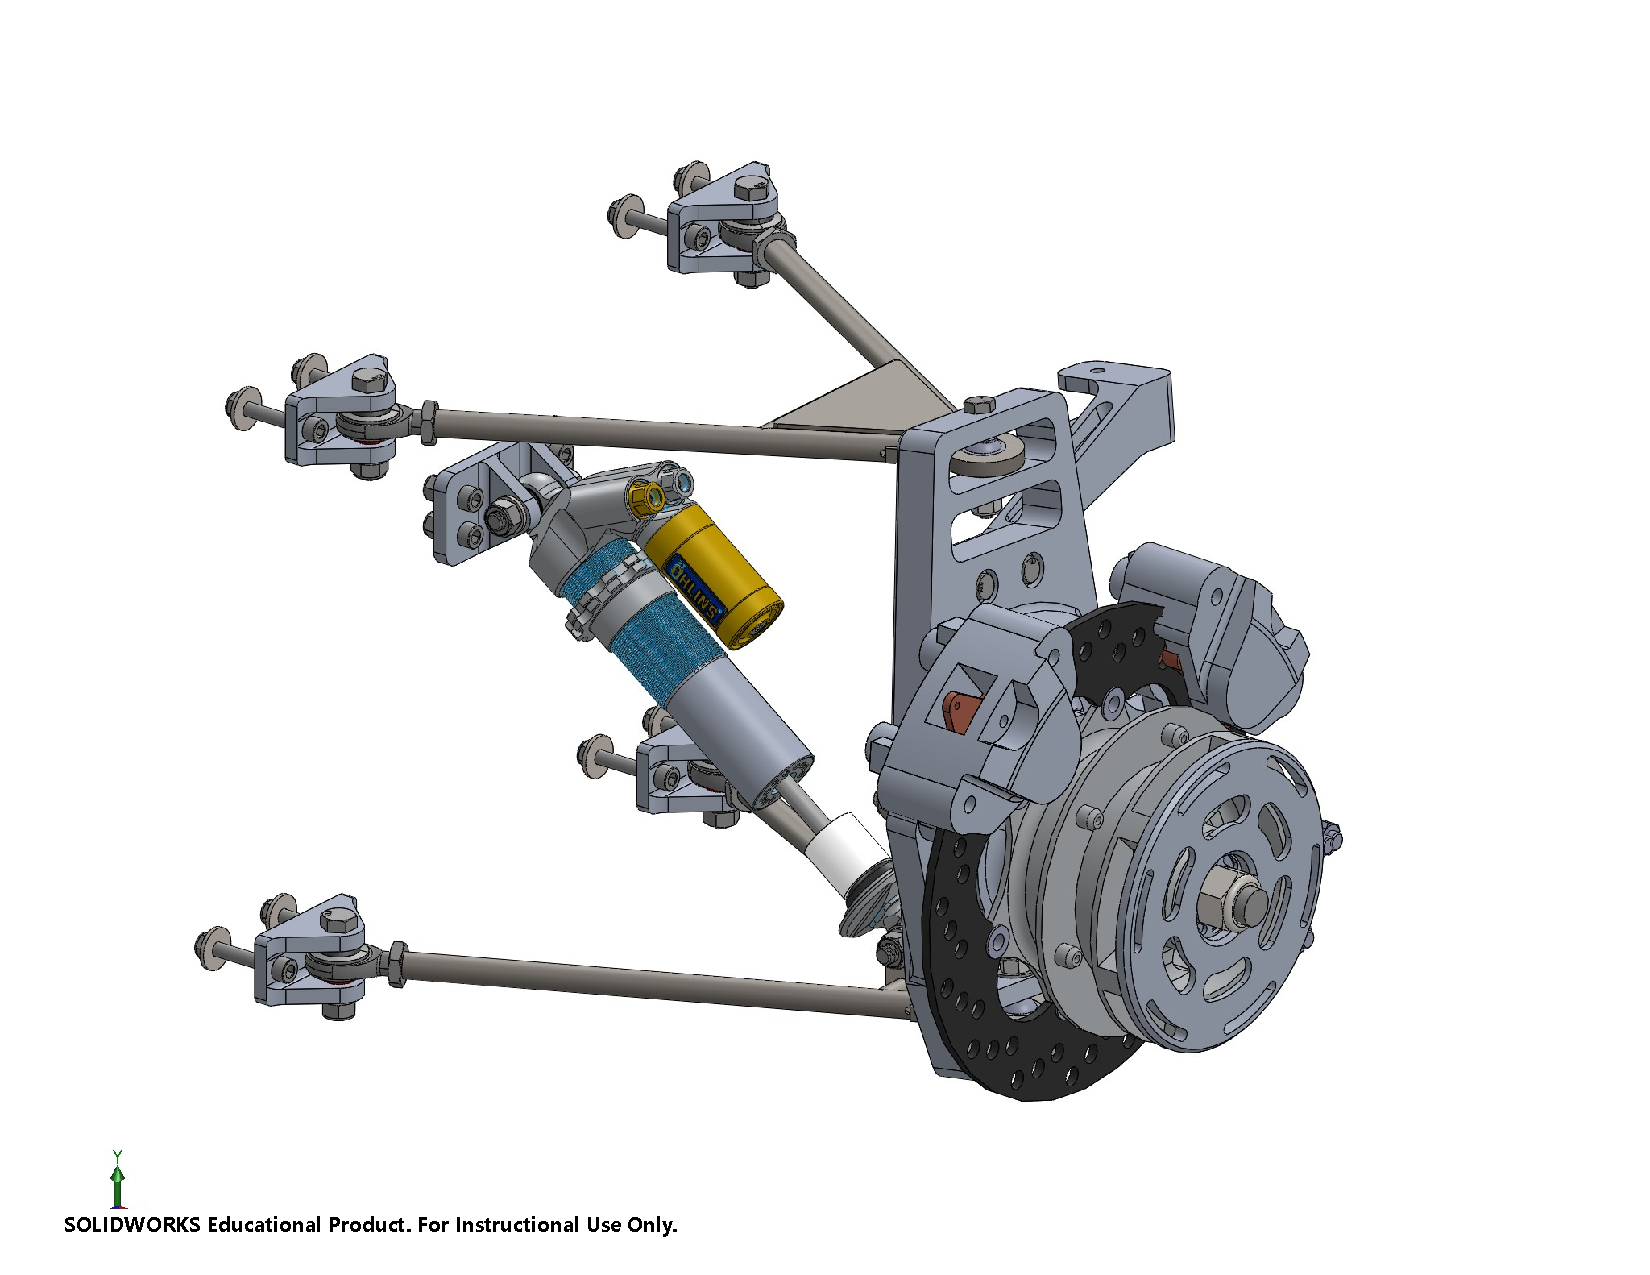
\includegraphics{figures/front-suspension}
\caption{View of front suspension assembly}
\label{fig:front-suspension}
\end{figure}

TODO: rod-end sizing justification based on shear loads

\subsubsection{Rear Suspension}
The rear suspension uses independent trailing arms mounted outwards from the rear of the chasssis. The trailing arm itself is custom-machined and mounts the same \"Ohlins TTX25 shock absorber as the front suspension. Figure \ref{fig:rear-suspension} shows the rear suspension assembly.

\begin{figure}
\centering
%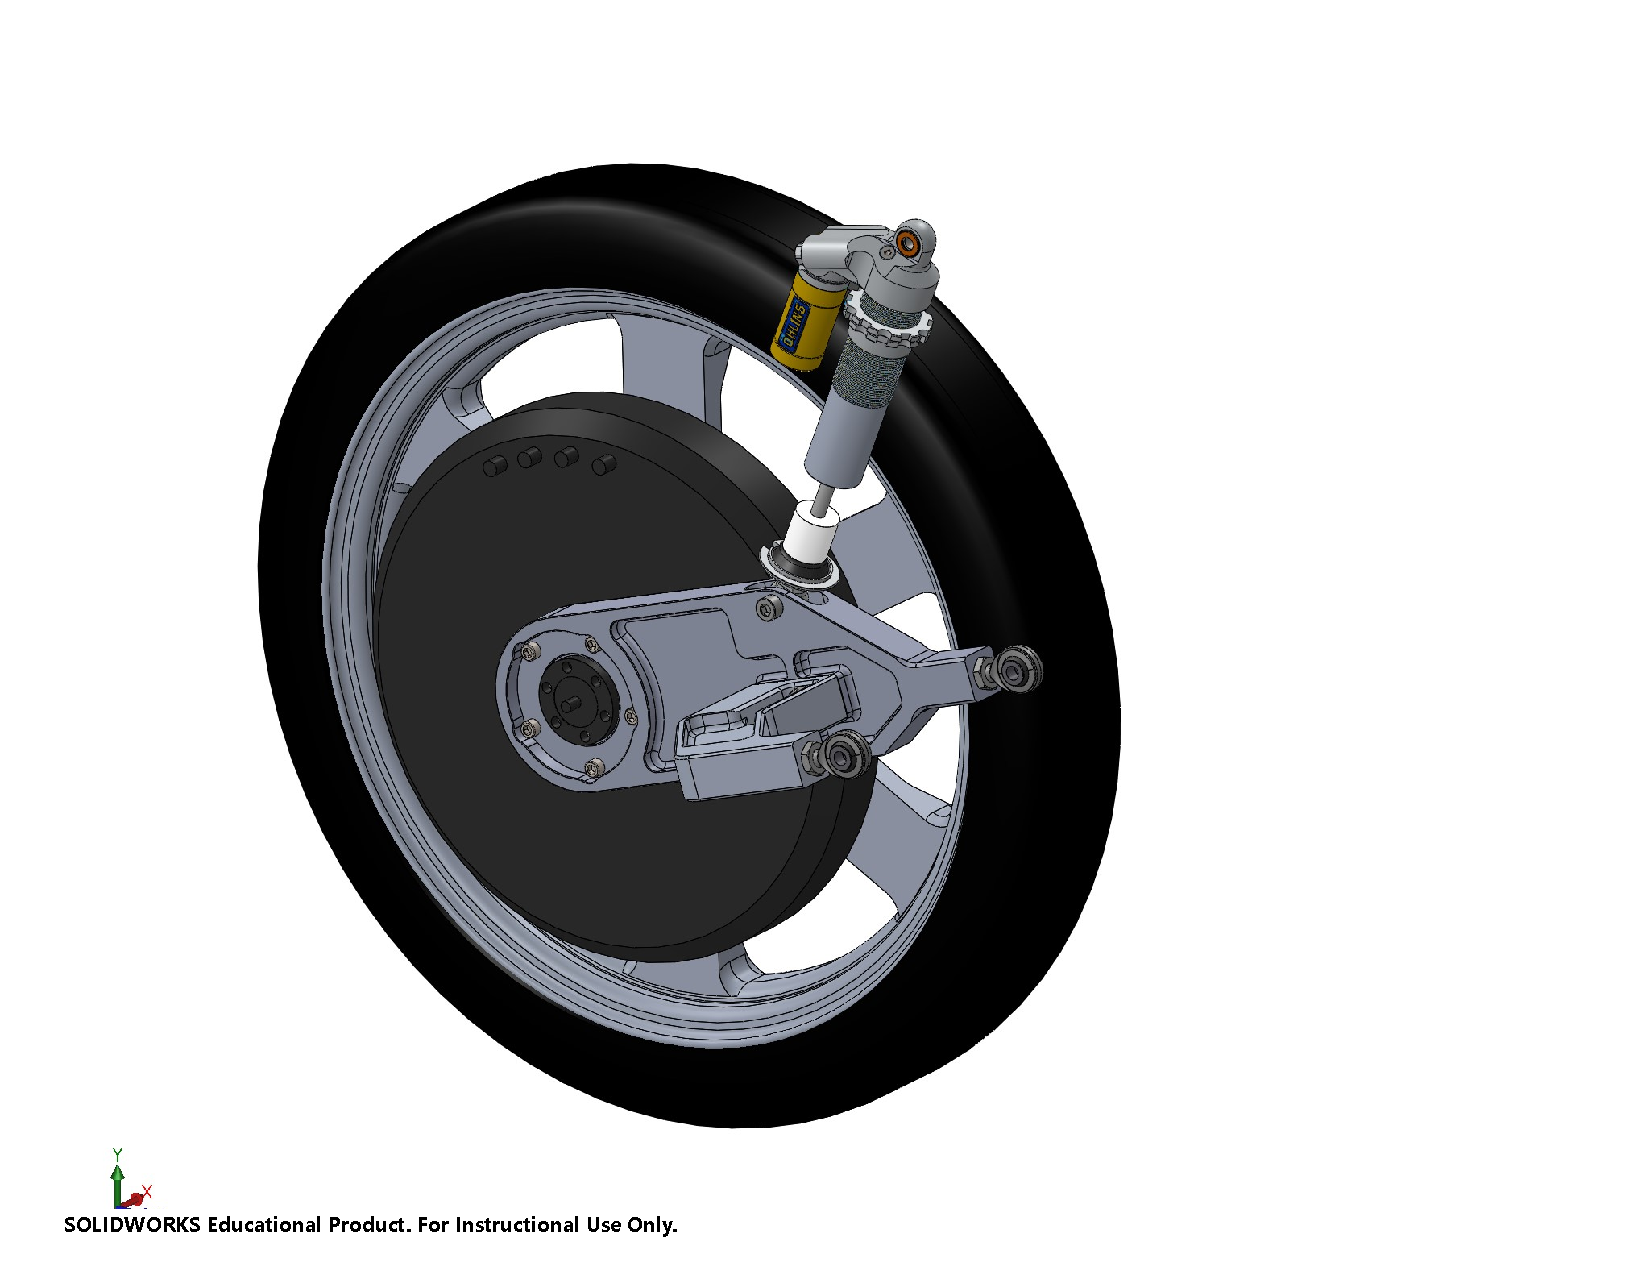
\includegraphics{figures/rear-suspension}
\caption{View of rear suspension assembly}
\label{fig:rear-suspension}
\end{figure}

TODO: rod-end sizing justification based on shear loads

\subsection{Structural Analysis}
FEA of suspension and steering components was done using ANSYS software. The specific loading conditions prescribed by ASC regulations are analyzed in this section.

\subsubsection{1G Turn}

\subsubsection{2G Bump}

\subsubsection{1G Braking}

\clearpage
\section{Electrical}


% Bibliography
%\pagebreak
%\printbibliography

% Appendix
%\pagebreak
%\appendix
%\section{Sample Appendix}
%\label{app:simple}
%\lstinputlisting[breaklines=true]{./matlab/script.m}
\end{document}
